\chapter{Xây dựng hệ thống và thiết lập thực nghiệm}
\label{sec:experimental-setup}

% Preamble: \usepackage{amsmath,amssymb,graphicx,booktabs,tabularx}.
% Đường dẫn mặc định khi biên dịch từ latex/; hỗ trợ workspace root.
\providecommand{\pcrauExpRoot}{../new}
\IfFileExists{new/test_iid/protocol/test_iid_eval_manifest.json}{%
    \renewcommand{\pcrauExpRoot}{new}}{}

Chương này trình bày cách hiện thực hóa phương pháp ở Chương~3 và
tổ chức thực nghiệm có thể kiểm tra lại bằng artifact. Nội dung tập trung
vào môi trường tính toán, bộ dữ liệu theo family, quy trình capture và
kiểm soát chất lượng, huấn luyện sidecar, khóa checkpoint, hiệu chuẩn và
đánh giá Test-IID. Các bảng sử dụng cấu hình, manifest và log thực trong
workspace; quy mô dự kiến hoặc thí nghiệm chưa chạy không được trình
bày như kết quả đã có.

Thí nghiệm hiện tại sử dụng P-CRA-U gồm V2 đóng băng, Adapter answerability và logistic33. Bộ Test-IID được capture sau khi khóa V2/calibrator ở vòng ban đầu; nay được dùng đánh giá lại Adapter. Bộ này đã từng được phân tích, không phải tập xác nhận mới chưa quan sát. Test-OOD không thuộc phạm vi đánh giá của khóa
luận này. Phần demo Gazebo được trình bày như kiểm chứng đường tích
hợp nhận thức, không đồng nhất với thành công pick-and-place.

Thiết kế đánh giá bám theo năm RQ ở Chương~1. RQ1 dùng so sánh grounding
paired với RoboRefer; RQ2 dùng phân bố không gian và metric answerability;
RQ3 dùng metric đa nhãn và thay đổi source score theo cặp family; RQ4 dùng
metric xác suất cùng coverage--area; RQ5 dùng lỗi trong tập chấp nhận và
audit đường tích hợp trước MoveIt. Cách tổ chức này phân biệt đánh giá
\emph{hiệu quả đầu ra} với đánh giá \emph{đóng góp riêng của kiến trúc}.
Loại thứ hai cần ablation có kiểm soát, được ghi riêng như phần còn thiếu.

\section{Hạ tầng và tổ chức phần mềm}
\label{sec:setup-infrastructure}

\subsection{Môi trường tính toán cho mô hình}

Huấn luyện và trích xuất đặc trưng được thực hiện trên máy có GPU
NVIDIA RTX 2000 Ada Generation, bộ nhớ khoảng 16~GB.
Artifact của run V2 lưu Python 3.10.14, PyTorch 2.5.1+cu124 và CUDA
runtime 12.4. Đây là thông tin tại thời điểm chạy thí nghiệm, cần
phân biệt với phiên bản thư viện có thể thay đổi trong môi trường
sau đó. Hệ điều hành đang sử dụng là Ubuntu 22.04 LTS.

Backbone RoboRefer-2B-SFT được lưu cục bộ; các tower RGB và depth
đóng băng tạo cache trước khi huấn luyện sidecar. Nhờ vậy, batch
huấn luyện không phải chứa toàn bộ quá trình sinh token của VLM.
Tuy nhiên, chi phí trích xuất tower vẫn phải được tính riêng khi
đánh giá độ trễ suy luận từ ảnh mới.

Dung lượng GPU khoảng 16~GB là cấu hình phần cứng, không phải VRAM đỉnh
đã đo của run. Báo cáo hiện chưa có bộ đo thống nhất về số tham số học
được, VRAM đỉnh, thời gian huấn luyện và latency end-to-end. Vì vậy,
khả năng huấn luyện trên cache là kết quả triển khai; ưu thế chi phí
hoặc tốc độ so với baseline chưa được kết luận định lượng.

\begin{table}[htbp]
    \centering
    \setlength{\tabcolsep}{4pt}
    \renewcommand{\arraystretch}{1.15}
    \caption{Môi trường tính toán và mô phỏng sử dụng trong đồ án.}
    \label{tab:setup-environment}
    \small
    \begin{tabularx}{\textwidth}{@{}>{\raggedright\arraybackslash}p{0.23\textwidth}>{\raggedright\arraybackslash}p{0.30\textwidth}>{\raggedright\arraybackslash}X@{}}
        \toprule
        Thành phần & Cấu hình & Vai trò/phạm vi \\
        \midrule
        GPU & RTX 2000 Ada, khoảng 16~GB &
        Trích xuất tower và huấn luyện sidecar \\
        Hệ điều hành & Ubuntu 22.04 LTS &
        Môi trường phát triển và mô phỏng \\
        Python & 3.10.14 & Phiên bản được ghi trong run V2 \\
        PyTorch / CUDA & 2.5.1+cu124 / 12.4 &
        Phiên bản được ghi trong run V2 \\
        ROS & ROS 2 Humble & Giao tiếp camera và hệ mô phỏng \\
        Gazebo & Fortress, dòng Ignition Gazebo 6 &
        Sinh quan sát RGB-D và nhãn đánh giá \\
        MoveIt & MoveIt 2 & Có trong môi trường; chưa nối vào
        cổng chấp hành best V2 đã xác minh \\
        Robot / gripper & UR3 / SusGrip 2F &
        Mô hình robot và gripper trong cảnh preview \\
        Camera & Mô hình D435i gắn cổ tay &
        Nguồn ảnh của giao thức capture; không phải đánh giá
        cảm biến vật lý ngoài đời \\
        \bottomrule
    \end{tabularx}
    \vspace{2pt}
    {\footnotesize\raggedright Nguồn: \texttt{run.json} của run V2, metadata môi
    trường cục bộ và tài liệu/code demo Gazebo trong workspace.\par}
\end{table}

\subsection{Môi trường mô phỏng và vai trò của các camera}

Gazebo được dùng để bố trí vật thể trên bàn và thu nhận RGB,
metric depth, thông tin camera cùng nhãn instance phục vụ evaluator.
UR3 và gripper trong preview giúp kiểm tra bố cục và góc nhìn,
nhưng robot tĩnh không chứng minh rằng một quỹ đạo đã được thực thi.

Trong giao thức Test-IID, đầu vào mô hình là RGB-D của camera cổ tay
ở pose khóa. Trong giao diện demo, camera ngoài có thể cung cấp góc
nhìn tổng thể từ bên trái robot, còn camera cổ tay cung cấp quan sát
cho suy luận. Ảnh tổng thể chỉ giúp người xem theo dõi; không được
âm thầm thay cho ảnh cổ tay rồi vẫn diễn giải risk như đã kiểm
chứng trên cùng miền Test-IID.

\subsection{Tách môi trường mô hình và môi trường ROS}

Các lệnh của mô hình đi qua script điều phối sử dụng môi trường
Python riêng và đường dẫn module của sidecar. Capture ROS sử
dụng các thành phần camera/bridge của môi trường mô phỏng.
Tách hai môi trường giảm xung đột phụ thuộc giữa PyTorch, thư
viện VLM và các gói ROS.

Script chạy đặt \texttt{PYTHONNOUSERSITE=1} để tránh nạp thư viện
người dùng ngoài môi trường đã chọn; đồng thời thiết lập
\texttt{PYTHONPATH} cho mã nguồn mới.
Seed được lưu trong cấu hình và dùng cho sampler/huấn luyện.
Các biện pháp này hỗ trợ tái lập, nhưng không tự bảo đảm bitwise
identical trên mọi GPU, phiên bản driver và kernel tính toán.

\subsection{Phân chia thư mục và trách nhiệm}

Code mới được đặt trong \texttt{new/}; dữ liệu và kết quả lịch sử
ở \texttt{old/} được đọc làm đầu vào. Kết quả run mới không ghi
đè dữ liệu lịch sử. Bảng~\ref{tab:setup-directory} mô tả các thành
phần chính, thay vì trộn model, dữ liệu, hình và checkpoint vào
một thư mục chung.

\begin{table}[htbp]
    \centering
    \setlength{\tabcolsep}{4pt}
    \renewcommand{\arraystretch}{1.15}
    \caption{Tổ chức các thành phần của hệ thống trong thư mục mới.}
    \label{tab:setup-directory}
    \small
    \begin{tabularx}{\textwidth}{@{}>{\raggedright\arraybackslash}p{0.28\textwidth}>{\raggedright\arraybackslash}X@{}}
        \toprule
        Thư mục trong \texttt{new/} & Nội dung chính \\
        \midrule
        \texttt{configs/} & Cấu hình V2 và các experiment V3 riêng \\
        \texttt{src/pcrau/} & Dataset, model, loss, hậu xử lý,
        metrics, calibrator và policy \\
        \texttt{scripts/} & Preflight, train, evaluate,
        calibrate, decide và các lệnh điều phối \\
        \texttt{tests/} & Kiểm thử hợp đồng dữ liệu, mô hình/loss,
        hậu xử lý, calibration/policy \\
        \texttt{outputs/} & Config snapshot, history,
        checkpoint và artifact theo từng run \\
        \texttt{test\_\allowbreak iid/} & Capture, materialization, feature cache,
        prediction và đánh giá Test-IID đã khóa \\
        \texttt{demo\_\allowbreak gazebo/} & Capture ROS, suy luận, dashboard
        và audit trước khi nối robot \\
        \texttt{hinhanh/} & Hình khoa học dựng từ artifact đã lưu \\
        \texttt{ketqua/} & Bộ kết quả được tập hợp theo nhóm để tra cứu \\
        \bottomrule
    \end{tabularx}
    \vspace{2pt}
    {\footnotesize\raggedright Nguồn: cấu trúc workspace và các entry point
    hiện có của hệ thống.\par}
\end{table}

\section{Bộ dữ liệu và quy trình thu nhận}
\label{sec:setup-dataset}

\subsection{Đơn vị family và sample}

Một family biểu diễn một kịch bản cảnh--truy vấn gốc cùng các biến
thể đối chứng. Mỗi family trong giao thức hiện tại có năm sample:
clean, semantic counterfactual, relation counterfactual, depth
corruption và occlusion/view counterfactual.

Sample không đồng nghĩa một ảnh RGB mới được chụp. Hai sample
có thể dùng cùng cặp ảnh nhưng khác câu lệnh; một sample depth
corruption có thể dùng cùng RGB nhưng một ảnh depth đã biến đổi.
Do đó, số sample, số capture vật lý trong mô phỏng và số cặp
feature duy nhất là ba đại lượng khác nhau.

Quan hệ phụ thuộc này cũng quyết định đơn vị chia tập và bootstrap.
Khóa luận không coi năm variant cùng family là năm quan sát
thống kê độc lập.

\subsection{Các tập dữ liệu sử dụng thực tế}

Dữ liệu development cũ có 400 family, chia cố định thành 320
train và 80 dev. Bộ calibration riêng có 200 family.
Test-IID được tạo mới với 200 family, không lấy 80 family dev
đổi tên thành test. Quy mô chính thức được tổng hợp ở
Bảng~\ref{tab:setup-splits}.

\begin{table}[htbp]
    \centering
    \setlength{\tabcolsep}{4pt}
    \renewcommand{\arraystretch}{1.15}
    \caption{Quy mô và vai trò của các tập dữ liệu trong thí nghiệm chính.}
    \label{tab:setup-splits}
    \small
    \begin{tabularx}{\textwidth}{@{}lrrr>{\raggedright\arraybackslash}X@{}}
        \toprule
        Tập & Family & Sample & \shortstack{Variant/\\family} & Vai trò \\
        \midrule
        Train & 320 & 1600 & 5 & Tối ưu tham số sidecar \\
        Dev & 80 & 400 & 5 & Chọn checkpoint và phân tích phát triển \\
        Calibration & 200 & 1000 & 5 &
        Fit calibrator/ngưỡng sau khi khóa checkpoint \\
        Test-IID & 200 & 1000 & 5 &
        Đánh giá V2 ban đầu; đánh giá lại Adapter trên IID cũ, không fit bằng test \\
        \midrule
        Tổng & 800 & 4000 & 5 &
        Bốn vai trò riêng; không gộp thành một tập huấn luyện \\
        \bottomrule
    \end{tabularx}
    \vspace{2pt}
    {\footnotesize\raggedright Nguồn: manifest development, calibration và
    evaluator Test-IID. Test-OOD không được sử dụng.\par}
\end{table}

Các quy mô prototype và candidate full trong kế hoạch chỉ là
mốc phát triển. Chúng không thay thế quy mô thực nghiệm được
báo cáo trong bảng trên. Run smoke cũng không được tính như
một bộ dữ liệu đánh giá bổ sung.

\subsection{Nhóm vật thể và ưu tiên của Test-IID}

Test-IID ưu tiên hoa quả, cốc và hộp, hạn chế cube làm target.
Cube vẫn có thể xuất hiện như distractor hoặc anchor.
Quota được đặt theo \emph{nhóm target chính của family}, không
phải thống kê số lần mọi vật xuất hiện trong ảnh.

\begin{table}[htbp]
    \centering
    \setlength{\tabcolsep}{4pt}
    \renewcommand{\arraystretch}{1.15}
    \caption{Quota nhóm vật đích chính của 200 family Test-IID.}
    \label{tab:setup-object-quota}
    \small
    \begin{tabularx}{\textwidth}{@{}lrr>{\raggedright\arraybackslash}X@{}}
        \toprule
        Nhóm & Family & Tỉ lệ (\%) & Ví dụ asset \\
        \midrule
        Hoa quả & 110 & 55.0 & Táo, cam, chanh và asset hoa quả khác \\
        Cốc & 30 & 15.0 & Mug \\
        Hộp & 20 & 10.0 & Cracker box, sugar box \\
        Chai/lon & 30 & 15.0 & Mustard bottle, tomato soup can \\
        Cube & 10 & 5.0 & Các cube màu trong registry \\
        \midrule
        Tổng & 200 & 100.0 & \\
        \bottomrule
    \end{tabularx}
    \vspace{2pt}
    {\footnotesize\raggedright Nguồn: quota trong generator và manifest
    Test-IID đã khóa. Variant thay câu lệnh có thể tham chiếu
    vật khác với target chính của family.\par}
\end{table}

Các asset được dùng trong cảnh mô phỏng; ảnh trong khóa luận
là ảnh render/capture Gazebo, không phải ảnh chụp robot vật lý.
Việc tăng tỉ lệ hoa quả làm bộ test gần nhu cầu demo hơn,
nhưng không có nghĩa đã có dữ liệu cho mọi lớp vật ngoài
registry hoặc mọi kiểu vật thể ngoài đời.

\subsection{Các kịch bản và phân bố answerability}

Sáu nhóm kịch bản gồm grounding trực tiếp, quan hệ 2D, trước/sau
theo camera, gần/xa, thứ tự chiều sâu đa anchor và thiếu bằng
chứng do che khuất/depth. Generator đặt 30, 40, 30, 35, 30 và
35 family cho các nhóm tương ứng, tổng cộng 200 family.

Trạng thái chuẩn của sample được lưu trong supervision.
Phân bố sau materialization không nên suy ra chỉ từ trạng thái
clean của family, vì counterfactual có thể đổi trạng thái.
Bảng~\ref{tab:setup-answer-distribution} thống kê tất cả variant.

\begin{table}[htbp]
    \centering
    \setlength{\tabcolsep}{4pt}
    \renewcommand{\arraystretch}{1.15}
    \caption{Phân bố nhãn answerability theo sample trên bốn tập.}
    \label{tab:setup-answer-distribution}
    \small
    \begin{tabularx}{\textwidth}{@{}>{\raggedright\arraybackslash}Xrrrr@{}}
        \toprule
        Nhãn & Train & Dev & Calibration & Test-IID \\
        \midrule
        \texttt{FOUND} & 673 & 168 & 420 & 420 \\
        \texttt{AMBIGUOUS} & 168 & 42 & 105 & 105 \\
        \texttt{ABSENT} & 211 & 53 & 132 & 132 \\
        \texttt{INSUFFICIENT\_\allowbreak EVIDENCE} & 548 & 137 & 343 & 343 \\
        \midrule
        Tổng & 1600 & 400 & 1000 & 1000 \\
        \bottomrule
    \end{tabularx}
    \vspace{2pt}
    {\footnotesize\raggedright Nguồn: nhãn supervision trong các manifest.
    Cùng phân bố lớp không đồng nghĩa calibration và test dùng
    cùng ảnh hoặc cùng family.\par}
\end{table}

\subsection{Capture RGB-D và annotation từ mô phỏng}

Mỗi capture lưu RGB gốc, metric depth, nhãn instance, thông tin
camera, TF snapshot và metadata. RGB, depth và nhãn được kiểm
tra tương ứng theo timestamp trước khi chấp nhận capture.
Đầu vào VLM chỉ dùng RGB/depth và câu lệnh; nhãn instance chỉ
được mở ở materializer/evaluator để tạo mask.

Target mask được tạo từ tập ID target hợp lệ theo câu lệnh.
Với trường hợp mơ hồ, mask có thể là hợp của nhiều ứng viên.
Target interior được tạo bằng erosion thích nghi, thử bán kính
tối đa 4 pixel và giảm nếu vùng còn quá nhỏ. Nếu không đạt mức
tối thiểu, hàm giữ mask gốc. Vì vậy, interior không được hiểu
là lúc nào cũng cách biên đúng 4 pixel.

Graspable/reachable mask trong materialization sử dụng heuristic
erosion, depth hợp lệ và vùng tọa độ bàn. Chúng là annotation
hỗ trợ evaluator, không phải xác nhận reachability bằng MoveIt.
Sự tồn tại các mask này không đủ để công bố tỉ lệ gắp thành công.

\begin{figure}[htbp]
    \centering
    \begin{minipage}{0.48\textwidth}
        \centering
        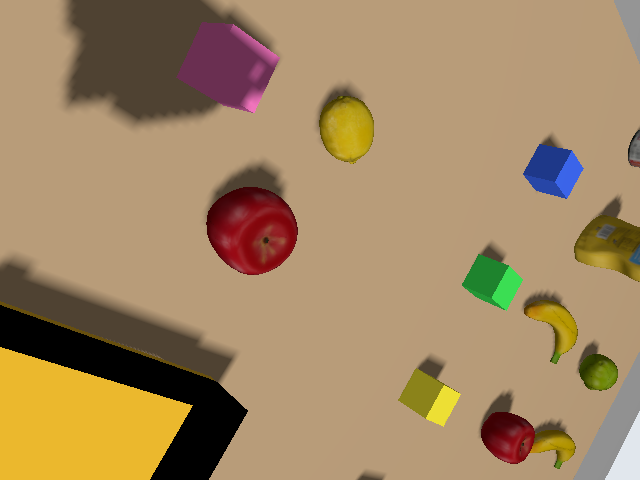
\includegraphics[width=\linewidth]{hinhanh/rgb.png}
        \par\small (a) RGB quan sát
    \end{minipage}\hfill
    \begin{minipage}{0.48\textwidth}
        \centering
        
\includegraphics[width=\linewidth]{hinhanh/depth_metric_visualization.png}
        \par\small (b) Metric depth trực quan hóa
    \end{minipage}
    \par\medskip
    \begin{minipage}{0.48\textwidth}
        \centering
        
\includegraphics[width=\linewidth]{hinhanh/semantic_instance_labels.png}
        \par\small (c) Nhãn instance của evaluator
    \end{minipage}\hfill
    \begin{minipage}{0.48\textwidth}
        \centering
        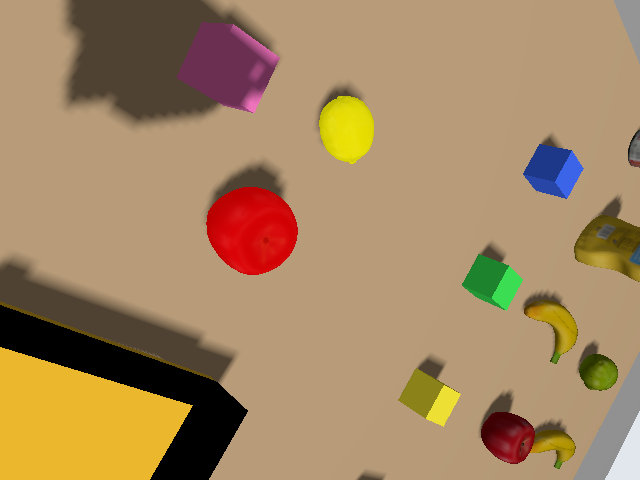
\includegraphics[width=\linewidth]{hinhanh/target_anchor_overlay.png}
        \par\small (d) Đối chiếu mask target--anchor
    \end{minipage}
    \caption{Ví dụ capture và annotation của một family trong canary
    Test-IID. Nhãn instance và overlay ở (c), (d) chỉ phục vụ
    kiểm tra/evaluator, không được đưa vào đầu vào mô hình.}
    \label{fig:setup-capture-annotation}
    {\footnotesize Nguồn: capture Gazebo và bộ bằng chứng QC thật
    của \texttt{v211iid\_\allowbreak family\_\allowbreak 000141} trong workspace.\par}
\end{figure}

\subsection{Thông số camera và hợp đồng cảm biến}

Giao thức capture khóa camera cổ tay, pose joint và giới hạn
chênh lệch timestamp. Bảng~\ref{tab:setup-camera} ghi thông số
từ capture plan; khi suy ngược 3D vẫn phải dùng camera info và
TF của capture tương ứng, không lấy một bộ số cố định thay
cho metadata của mọi cảnh.

\begin{table}[htbp]
    \centering
    \setlength{\tabcolsep}{4pt}
    \renewcommand{\arraystretch}{1.15}
    \caption{Thông số camera trong kế hoạch capture Test-IID đã khóa.}
    \label{tab:setup-camera}
    \small
    \begin{tabularx}{\textwidth}{@{}>{\raggedright\arraybackslash}p{0.32\textwidth}>{\raggedright\arraybackslash}X@{}}
        \toprule
        Đại lượng & Giá trị/quy ước \\
        \midrule
        Độ phân giải RGB/depth & $640\times480$ pixel \\
        $(f_x,f_y)$ & $(606.081665,\ 605.797302)$ pixel \\
        $(c_x,c_y)$ & $(325.543671,\ 249.996155)$ pixel \\
        Đơn vị metric depth & Mét \\
        Chênh lệch timestamp tối đa & 0.035~s \\
        RGB topic & \texttt{/wrist\_\allowbreak camera/color/image\_\allowbreak raw} \\
        Depth topic & \texttt{/wrist\_\allowbreak camera/depth/image\_\allowbreak raw} \\
        Pose sáu joint, rad &
        $(1.7315,-2.0273,1.2428,-1.5363,-1.5708,-1.9601)$ \\
        \bottomrule
    \end{tabularx}
    \vspace{2pt}
    {\footnotesize\raggedright Nguồn: \texttt{test\_\allowbreak iid\_\allowbreak capture\_\allowbreak plan.json}.
    Pose là cấu hình capture, không phải lệnh chuyển động do V2 sinh ra.\par}
\end{table}

\section{Chia tập, tính độc lập và khóa dữ liệu}
\label{sec:setup-split-policy}

\subsection{Chia theo family thay vì sample}

Tập train và dev được lấy từ manifest development đã có,
không chia ngẫu nhiên lại ở mỗi lần train. Điều kiện bắt buộc là
\begin{equation}
    \mathcal{F}_{\mathrm{train}}\cap
    \mathcal{F}_{\mathrm{dev}}=\varnothing,
    \qquad
    \operatorname{split}(x_{f,v})=\operatorname{split}(f).
\end{equation}
Toàn bộ variant của một family ở cùng tập. Nếu chia theo
sample, ảnh sạch của một cảnh có thể vào train còn câu lệnh
đối chứng trên chính ảnh đó vào dev; kết quả sẽ bị lạc quan.

Calibration và Test-IID có namespace family riêng. Kiểm tra
không trùng family ID cần đi kèm kiểm tra nội dung: đổi tên ID
không đủ nếu ảnh, layout hoặc capture cũ được dùng lại.
Preflight Test-IID đối chiếu với lịch sử capture/layout/
instruction, và QC materialized kiểm tra hash RGB/depth.

\subsection{Quan hệ giữa IID và giới hạn khái quát hóa}

Test-IID giữ registry asset, cấu trúc mẫu câu, cách tiền xử lý
và quy ước quan hệ tương thích với giao thức development,
đồng thời dùng family, layout và capture mới.
IID ở đây là phạm vi đánh giá trong giao thức mô phỏng,
không phải khẳng định mọi ảnh robot sau này đều cùng phân bố.

Quota nhóm vật đích được ưu tiên lại cho hoa quả/cốc/hộp,
nên cần ghi rõ composition của test khi diễn giải kết quả.
Một dashboard có pose tương tự Test-IID nhưng bố cục tùy
chỉnh vẫn không trở thành một sample Test-IID chính thức.
Khóa luận không sử dụng Test-OOD; vì thế các kết luận không
bao gồm khả năng chống mọi domain shift hoặc chuyển sang
robot vật lý chưa đo.

\subsection{Tách manifest inference và evaluator}

Test-IID có hai manifest: feature manifest chứa đường dẫn
RGB/depth và câu lệnh, còn eval manifest chứa supervision,
mask và thông tin audit. Hai manifest liên kết bằng
\texttt{sample\_\allowbreak id}, nhưng không được nạp theo cùng quyền
trong runner suy luận gốc.

Ở training/evaluation sidecar, batch có thể chứa nhãn để
tính loss và chỉ số; trước khi gọi forward, code chỉ chọn
tập input hợp lệ. Nhãn không được ghép vào feature tensor,
token hay vector evidence. Prediction thô được lưu trước
khi tổng hợp các phân tích có ground-truth.

\subsection{Mã băm và trạng thái khóa}

Checkpoint, calibrator, model inventory, manifest và một số
script được ghi SHA-256 trong lock artifact. Test-IID phải
vượt qua hai cổng khác nhau: cổng cho phép capture và cổng
cho phép suy luận sau materialization/QC. Lock ban đầu có
trạng thái không cho phép suy luận là dấu vết lịch sử,
không có nghĩa kết quả test hiện tại chưa được chạy.

Sau cổng suy luận đóng băng, không được fit lại calibrator,
chọn ngưỡng source/risk hoặc chỉnh prompt bằng kết quả test
rồi báo cáo cùng bộ đó như đánh giá chưa từng sử dụng.
Nếu cần một vòng phát triển mới, phải tách rõ experiment
và cách xử lý bộ test đã được xem.

\section{Dữ liệu counterfactual và kiểm soát chất lượng}
\label{sec:setup-counterfactual}

\subsection{Năm variant trong mỗi family}

Thiết kế đối chứng giúp phân tích phản ứng của mô hình khi
câu lệnh hoặc bằng chứng quan sát thay đổi. Bảng~\ref{tab:setup-variants}
tóm tắt vai trò của năm variant. “Clean” chỉ là variant tham chiếu
không có perturbation bổ sung theo nhánh đối chứng; clean vẫn có
thể thuộc trạng thái absent, ambiguous hoặc insufficient evidence.
Không được coi toàn bộ clean là \texttt{FOUND}.

\begin{table}[htbp]
    \centering
    \setlength{\tabcolsep}{4pt}
    \renewcommand{\arraystretch}{1.15}
    \caption{Vai trò các variant trong giao thức scene--query family.}
    \label{tab:setup-variants}
    \small
    \begin{tabularx}{\textwidth}{@{}>{\raggedright\arraybackslash}p{0.22\textwidth}>{\raggedright\arraybackslash}p{0.28\textwidth}>{\raggedright\arraybackslash}X@{}}
        \toprule
        Variant & Thành phần thay đổi & Mục đích đối chứng \\
        \midrule
        Clean & Kịch bản tham chiếu của family &
        Mốc so sánh; có đủ bốn trạng thái answerability \\
        Semantic CF & Tham chiếu/ngữ nghĩa trong câu lệnh &
        Kiểm tra tác động của mô tả vật đích trên cùng quan sát \\
        Relation CF & Điều kiện quan hệ trong câu lệnh &
        Kiểm tra ràng buộc không gian, không chỉ tên vật \\
        Depth corruption & Relative depth đầu vào &
        Đo phản ứng khi bằng chứng depth suy giảm hoặc xung đột \\
        Occlusion/view CF & Capture bổ sung theo plan &
        Kiểm tra thay đổi bằng chứng nhìn thấy/che khuất \\
        \bottomrule
    \end{tabularx}
    \vspace{2pt}
    {\footnotesize\raggedright Nguồn: variant specs trong manifest và code
    materialization. CF: counterfactual.\par}
\end{table}

Semantic/relation counterfactual không nhất thiết làm câu
lệnh vô nghiệm. Một câu lệnh đã thay đổi có thể vẫn chọn
được một vật khác. Nhãn answerability và source vì vậy lấy
từ supervision thực của từng variant, không đặt nhãn dương
chỉ vì tên variant có chữ counterfactual.

\subsection{Các phép gây nhiễu depth đã sử dụng}

Trên 200 sample mang tên depth corruption của Test-IID,
manifest phân bổ ba phép gây nhiễu như
Bảng~\ref{tab:setup-depth-corruption}. Các phép này tác động
lên ảnh relative depth đã chuẩn hóa; metric depth gốc
được giữ riêng để kiểm tra và truy vết.

\begin{table}[htbp]
    \centering
    \setlength{\tabcolsep}{4pt}
    \renewcommand{\arraystretch}{1.15}
    \caption{Các loại depth corruption trong 200 variant đối chứng Test-IID.}
    \label{tab:setup-depth-corruption}
    \small
    \begin{tabularx}{\textwidth}{@{}>{\raggedright\arraybackslash}p{0.23\textwidth}r>{\raggedright\arraybackslash}X@{}}
        \toprule
        Loại & Sample & Hiện thực hóa \\
        \midrule
        Bias/noise & 76 &
        Cộng bias xám 14 và nhiễu Gaussian $\sigma=5$,
        chặn kết quả trong $[0,255]$ \\
        Local holes/edges & 63 &
        Tạo vùng mất giá trị quanh biên depth và các vùng
        cục bộ; đặt pixel bị ảnh hưởng bằng 0 \\
        Inversion/shift & 61 &
        Đảo mức xám $255-Z_{\mathrm{rel}}$ và dịch vòng
        $(\Delta y,\Delta x)=(9,-13)$ pixel \\
        \midrule
        Tổng & 200 & Một depth-corruption variant cho mỗi family \\
        \bottomrule
    \end{tabularx}
    \vspace{2pt}
    {\footnotesize\raggedright Nguồn: perturbation specs của Test-IID và
    hàm \texttt{corrupt\_\allowbreak depth} trong materializer.\par}
\end{table}

Ngoài nhánh đối chứng trên, một số clean có submode depth
hỏng hoặc xung đột đa phương thức. Trong Test-IID, 16 clean
dùng local holes/edges và 7 clean dùng cross-modal shift
ngang 37 pixel. Vì vậy, số sample bị sửa depth không chỉ
là 200 sample có tên \texttt{depth\_\allowbreak corruption}.

Phép dịch trong code dùng dịch vòng; đây là perturbation
tổng hợp để khảo sát độ nhạy, không phải mô phỏng đầy đủ
nhiễu vật lý của camera D435i. Các biến thể flat, shuffled
hoặc missing toàn bộ depth nêu trong thiết kế mục tiêu
không được báo như nhóm thí nghiệm chính đã có của Test-IID
hiện tại. Chức năng stripe dropout có trong helper cũng
không đồng nghĩa có sample chính thức sử dụng nó.

\subsection{Phân bố relation theo variant}

Bảng~\ref{tab:setup-relation-distribution} ghi nhãn relation
vận hành của từng sample. Mỗi sample đóng góp một nhãn
audit relation trong bảng này; bảng không phải thống kê
số cạnh ngữ nghĩa của mọi mệnh đề trong câu.
Counterfactual có thể đổi relation, nên phân bố sau
materialization khác quota kịch bản ở cấp family.

\begin{table}[htbp]
    \centering
    \setlength{\tabcolsep}{4pt}
    \renewcommand{\arraystretch}{1.15}
    \caption{Phân bố nhãn relation vận hành trên các tập dữ liệu.}
    \label{tab:setup-relation-distribution}
    \small
    \begin{tabularx}{\textwidth}{@{}>{\raggedright\arraybackslash}Xrrrr@{}}
        \toprule
        Relation & Train & Dev & Calibration & Test-IID \\
        \midrule
        \texttt{direct} & 560 & 140 & 350 & 350 \\
        \texttt{left\_\allowbreak of} & 120 & 30 & 76 & 78 \\
        \texttt{right\_\allowbreak of} & 136 & 34 & 84 & 82 \\
        \texttt{front\_\allowbreak of} & 266 & 68 & 165 & 169 \\
        \texttt{behind} & 150 & 36 & 95 & 91 \\
        \texttt{nearer\_\allowbreak than} & 116 & 26 & 67 & 73 \\
        \texttt{farther\_\allowbreak than} & 108 & 30 & 73 & 67 \\
        \texttt{between\_\allowbreak in\_\allowbreak depth} & 51 & 21 & 33 & 42 \\
        \texttt{nearer\_\allowbreak than\_\allowbreak both} & 93 & 15 & 57 & 48 \\
        \midrule
        Tổng & 1600 & 400 & 1000 & 1000 \\
        \bottomrule
    \end{tabularx}
    \vspace{2pt}
    {\footnotesize\raggedright Nguồn: trường \texttt{audit\_\allowbreak only.relation}
    trong manifest development, calibration và eval Test-IID.\par}
\end{table}

\subsection{Phân bố source uncertainty và nhãn yếu}

Source là bài toán đa nhãn. Bảng~\ref{tab:setup-source-distribution}
ghi số sample dương của từng source; tổng các hàng không cần
bằng số sample. Nhãn spatial được suy từ \texttt{AMBIGUOUS}
theo quy tắc đã công bố, không phải nhãn nhân quả bổ sung
do evaluator đo độc lập.

\begin{table}[htbp]
    \centering
    \setlength{\tabcolsep}{4pt}
    \renewcommand{\arraystretch}{1.15}
    \caption{Số nhãn dương theo source uncertainty trên bốn tập.}
    \label{tab:setup-source-distribution}
    \small
    \begin{tabularx}{\textwidth}{@{}>{\raggedright\arraybackslash}Xrrrr@{}}
        \toprule
        Source & Train & Dev & Calibration & Test-IID \\
        \midrule
        Semantic & 379 & 95 & 237 & 237 \\
        Relation & 379 & 95 & 237 & 237 \\
        Spatial (nhãn yếu) & 168 & 42 & 105 & 105 \\
        Depth & 272 & 67 & 164 & 160 \\
        Occlusion & 276 & 70 & 179 & 183 \\
        \bottomrule
    \end{tabularx}
    \vspace{2pt}
    {\footnotesize\raggedright Nguồn: source labels trong manifest; spatial
    được tính theo \texttt{answerability == AMBIGUOUS}.
    Các hàng không loại trừ nhau.\par}
\end{table}

Số positive depth/occlusion khác số variant cùng tên do
quy tắc nhãn còn phụ thuộc trạng thái và mức bằng chứng.
Đánh giá source theo tên variant thay vì nhãn supervision
sẽ thay đổi bài toán và có thể tạo ra false positive/false
negative giả.

\subsection{Canary trước khi capture toàn bộ Test-IID}

Capture bắt đầu bằng canary 20 family/40 capture. Sau khi
QC đạt, hệ thống mới chuyển sang hai batch 90 family,
mỗi batch 180 capture. Tổng là 200 family/400 capture.
Một family sử dụng capture tham chiếu và capture
occlusion bổ sung; từ đó materializer tạo năm variant.

QC kiểm tra số lượng và danh tính capture, mã băm, decode
ảnh, kích thước/dtype, độ hợp lệ depth, mức đồng bộ timestamp,
quan hệ quan sát được và tình trạng shutdown.
QC không sử dụng prediction của V2 để lựa chọn giữ lại các
ảnh mô hình làm đúng. Cổng chất lượng dữ liệu phải được
đánh giá trước khi mở suy luận.

\begin{table}[htbp]
    \centering
    \setlength{\tabcolsep}{4pt}
    \renewcommand{\arraystretch}{1.15}
    \caption{Kết quả kiểm soát chất lượng ba batch capture Test-IID.}
    \label{tab:setup-capture-qc}
    \small
    \begin{tabularx}{\textwidth}{@{}>{\raggedright\arraybackslash}Xrrrrc@{}}
        \toprule
        Batch & Family & Capture & \shortstack{$\Delta t_{\max}$\\(ms)} & \shortstack{Depth hợp lệ\\(\%)} & QC \\
        \midrule
        Canary & 20 & 40 & 33.0 & 99.601 & Đạt \\
        Batch 1 & 90 & 180 & 33.0 & 98.926 & Đạt \\
        Batch 2 & 90 & 180 & 33.0 & 98.848 & Đạt \\
        \midrule
        Tổng & 200 & 400 & & & Đạt \\
        \bottomrule
    \end{tabularx}
    \vspace{2pt}
    {\footnotesize\raggedright Nguồn: ba báo cáo \texttt{batch\_\allowbreak qc}.
    Depth hợp lệ là trung bình tỉ lệ pixel hợp lệ của batch;
    không phải độ chính xác đo depth. Giới hạn $\Delta t$ là 35~ms.\par}
\end{table}

\subsection{Materialization và xử lý gián đoạn}

Sau đủ 400 capture, materializer kiểm tra toàn bộ plan,
danh tính capture và hash trước khi tạo 1000 record.
Record liên kết ảnh đầu vào, câu lệnh, perturbation,
metadata cảm biến và evaluator-only mask.
Ảnh RGB đầu vào được ghi JPEG chất lượng 95; relative
depth lưu PNG; metric depth giữ dạng mảng float32.

Capture có checkpoint sau từng family và ở biên batch.
Khi tiếp tục sau gián đoạn, capture hoàn chỉnh chỉ được
bỏ qua sau khi xác minh mọi hash được khai báo. Capture
thiếu hoặc hỏng gây dừng để xử lý, không tự ghi đè.
Quy tắc này giúp phân biệt dữ liệu đã thu nhận với dữ
liệu mới sau khi mất điện hoặc tiến trình bị ngắt.

Báo cáo materialized xác nhận 1000 sample, 200 family,
và không trùng hash RGB/depth với development/calibration
theo các kiểm tra đã thực hiện. Nó không thay thế kiểm
tra toàn bộ mọi hình thức tương đồng ngữ nghĩa giữa
các cảnh; phạm vi kiểm tra cần được ghi đúng như artifact.

\section{Các giai đoạn huấn luyện và khóa mô hình}
\label{sec:setup-training}

\subsection{Hợp đồng đặc trưng và feature cache}

Cache chứa bốn tensor có tên cố định:
\texttt{R0\_\allowbreak GRID}, \texttt{D0\_\allowbreak GRID},
\texttt{R0\_\allowbreak THUMB}, \texttt{D0\_\allowbreak THUMB}.
Hai tensor lưới có shape $24\times32\times1152$,
hai thumbnail có shape $1152$.
Tên tensor, shape và cấu hình pooling là hợp đồng đầu
vào, không được thay bằng feature tương tự kích thước
nhưng có ý nghĩa khác.

Index development có 1242 cặp feature duy nhất cho
2000 sample, calibration có 618 cặp cho 1000 sample,
Test-IID có 619 cặp cho 1000 sample.
Feature có thể dùng chung khi RGB và depth giống nhau,
còn token câu lệnh vẫn được xử lý riêng.
Cache là cơ chế giảm tính toán, không phải cơ chế tăng
số mẫu độc lập.

Cache Test-IID lưu float16; dataset chuyển feature
sang float32 trước đường tính toán của sidecar, rồi
autocast có thể dùng bfloat16 trong các phép toán phù
hợp. Cần phân biệt dtype lưu trữ với dtype thực thi.
Khi tái dùng cache, code kiểm tra SHA-256, tên tensor,
shape, dtype và giá trị hữu hạn theo hợp đồng.

\subsection{Quy trình T0--T5}

Các giai đoạn được tách theo quyền truy cập dữ liệu:
kiểm tra hợp đồng, smoke, development training,
candidate freeze, calibration và locked evaluation.
Bảng~\ref{tab:setup-training-stages} ghi cách thực hiện
trong workspace.

\begin{table}[htbp]
    \centering
    \setlength{\tabcolsep}{4pt}
    \renewcommand{\arraystretch}{1.15}
    \caption{Các giai đoạn từ kiểm thử kỹ thuật đến đánh giá khóa.}
    \label{tab:setup-training-stages}
    \small
    \begin{tabularx}{\textwidth}{@{}l>{\raggedright\arraybackslash}p{0.23\textwidth}>{\raggedright\arraybackslash}X@{}}
        \toprule
        Mốc & Dữ liệu/phạm vi & Thao tác và artifact \\
        \midrule
        T0 & Manifest/cache &
        Preflight số family/variant, tensor contract,
        file và hash; không huấn luyện backbone \\
        T1 & Batch phát triển nhỏ &
        Smoke một train batch và một dev batch; kiểm
        tra forward/loss/update/save/load \\
        T2 & Train và dev &
        Huấn luyện sidecar đa nhiệm; lưu history và
        chọn best theo dev total loss \\
        T3 & Candidate từ dev &
        Khóa V2 epoch 13/step 1120, config và model hash \\
        T4 & Calibration riêng &
        Suy luận đóng băng, fit logistic, chọn ngưỡng
        risk và khối lượng vùng tin cậy \\
        T5 & Test-IID độc lập &
        Capture/QC, khóa inference, đánh giá V2 và
        RoboRefer trên cùng sample, bootstrap theo family \\
        \bottomrule
    \end{tabularx}
    \vspace{2pt}
    {\footnotesize\raggedright Nguồn: entry point, run artifact và lock
    Test-IID. Smoke không thay thế thử nghiệm overfit
    nhỏ đạt một tiêu chí định lượng.\par}
\end{table}

Artifact smoke hiện có chỉ chứa một optimizer step.
Nó chứng minh đường chạy kỹ thuật có thể hoạt động,
không chứng minh mô hình đã học đủ hoặc đạt hiệu quả
định lượng. Thử nghiệm overfit cần tiêu chí hội tụ
riêng; không suy ra từ tên thư mục smoke.

\subsection{Hyperparameter của baseline V2}

Sidecar được khởi tạo và huấn luyện trên feature đóng
băng, không resume optimizer của một experiment V3.
Cấu hình chính được trình bày trong
Bảng~\ref{tab:setup-v2-hyperparameters}.

Tokenizer sidecar chuyển chữ thường, tách token chữ/số theo mẫu tiếng
Anh và giữ tối đa 72 token. Với vocabulary 8192, ánh xạ dùng
$\operatorname{id}(w)=1+(\operatorname{hash}_{64}(w)\bmod8191)$,
trong đó $\operatorname{hash}_{64}$ lấy từ SHA-256; ID 0 dành cho padding.
Câu rỗng nhận một token dự phòng. Quy tắc này được giữ cố định cùng
config để tái lập input của bộ mã hóa truy vấn ở Chương~3.

\begin{table}[htbp]
    \centering
    \setlength{\tabcolsep}{4pt}
    \renewcommand{\arraystretch}{1.15}
    \caption{Hyperparameter của run baseline V2.}
    \label{tab:setup-v2-hyperparameters}
    \small
    \begin{tabularx}{\textwidth}{@{}>{\raggedright\arraybackslash}p{0.45\textwidth}>{\raggedright\arraybackslash}X@{}}
        \toprule
        Tham số & Giá trị \\
        \midrule
        Seed & 24082026 \\
        Optimizer & AdamW \\
        Learning rate ban đầu & $2\times10^{-4}$ \\
        Weight decay & $10^{-4}$ \\
        Scheduler & Warmup tuyến tính, sau đó cosine decay \\
        Warmup & 200 optimizer step \\
        Số epoch cấu hình & 20 \\
        Early-stopping patience & 6 epoch \\
        Family/batch & 4 \\
        Sample/batch & 20, đủ năm variant/family \\
        Batch/epoch & 80 \\
        Gradient clip norm & 5.0 \\
        Mixed precision & Bfloat16 autocast \\
        DataLoader worker & 0 \\
        Hidden dimension & 128 \\
        Text/fusion layer & 2 / 2 \\
        Attention head ở text/query & 4 \\
        Dropout & 0.1 \\
        Modality dropout & Không kích hoạt trong baseline V2 \\
        Số token tối đa / vocabulary & 72 / 8192 \\
        Số relation/anchor slot tối đa & 3 / 3 \\
        Tiêu chí chọn checkpoint & Dev total loss thấp nhất \\
        Chu kỳ checkpoint định kỳ & 1 epoch trong run V2 \\
        \bottomrule
    \end{tabularx}
    \vspace{2pt}
    {\footnotesize\raggedright Nguồn: config snapshot của
    \texttt{pcrau\_\allowbreak target\_\allowbreak v2\_\allowbreak full\_\allowbreak seed\_\allowbreak 24082026}
    và script training. Best được cập nhật riêng khi dev cải thiện.\par}
\end{table}

{\setlength{\emergencystretch}{3em}
Mỗi epoch có 80 batch do $320/4=80$ family-complete
batch, tương ứng 1600 sample presentation. Không có
oversampling của experiment V3 trong run này.
Trọng số loss target/interior/anchor/edge/answer/source/
ranking lần lượt là
$(1.0,0.4,0.6,0.4,0.7,0.5,0.2)$, ranking margin 0.25
trên logits và trọng số spatial weak label 0.5.
Các công thức đã trình bày ở Chương~3 không được thay
bằng loss khác khi diễn giải run đã hoàn tất.\par}


\subsection{Logging và chọn checkpoint tốt nhất}

History lưu epoch, global step, learning rate,
loss train, loss dev và các metric dev.
\texttt{train\_\allowbreak total} là tổng loss trên train;
\texttt{dev\_\allowbreak total} là tổng loss dev; \texttt{best}
là giá trị tiêu chí chọn checkpoint tốt nhất tính
đến thời điểm đó. Chúng không phải phần trăm accuracy.

Epoch trong artifact đánh số từ 0. Vì vậy,
\texttt{epoch=13} là cuối lượt epoch thứ 14 nếu đếm
bắt đầu từ 1; $14\times80=1120$ optimizer step.
History V2 có 20 bản ghi, từ epoch 0 đến 19.
Việc chọn epoch 13 không có nghĩa toàn run chỉ
huấn luyện 13 epoch.

\begin{table}[htbp]
    \centering
    \setlength{\tabcolsep}{4pt}
    \renewcommand{\arraystretch}{1.15}
    \caption{Thông tin định danh best checkpoint V2 được dùng cho Test-IID.}
    \label{tab:setup-best-checkpoint}
    \small
    \begin{tabularx}{\textwidth}{@{}>{\raggedright\arraybackslash}p{0.43\textwidth}>{\raggedright\arraybackslash}X@{}}
        \toprule
        Trường & Giá trị \\
        \midrule
        Epoch lưu trong metadata & 13, chỉ số bắt đầu từ 0 \\
        Global optimizer step & 1120 \\
        Tập chọn checkpoint & Dev, 80 family/400 sample \\
        Selected dev total loss & 1.697110856 \\
        Train total loss tại checkpoint & 1.172486611 \\
        LR cuối epoch tương ứng & $5.261313375\times10^{-5}$ \\
        Model SHA-256, 16 ký tự đầu & \texttt{1505152fca7b725d} \\
        Config SHA-256, 16 ký tự đầu & \texttt{e4f21ccc255c2f09} \\
        Calibrator SHA-256, 16 ký tự đầu & \texttt{f4ed0abb06ed9628} \\
        \bottomrule
    \end{tabularx}
    \vspace{2pt}
    {\footnotesize\raggedright Nguồn: \texttt{best.json}, metadata checkpoint
    và freeze lock. Hash đầy đủ nằm trong artifact;
    LR tại epoch không phải LR ban đầu.\par}
\end{table}

\subsection{Lưu trạng thái và tiếp tục huấn luyện}

Mỗi checkpoint gồm model safetensors, trainer state
và metadata. Trainer state lưu optimizer, scheduler,
epoch, global step và best metric. Load model kiểm
tra hash, config hash và state dict với chế độ strict.
Resume phải trỏ vào đúng run đã chọn và đúng config.

Đường resume hiện tại không lưu đầy đủ trạng thái
RNG hay toàn bộ trạng thái early stopping. Vì thế,
resume từ một checkpoint hợp lệ giúp tiếp tục tối
ưu nhưng không được tuyên bố tương đương bitwise với
một run chưa từng bị ngắt. Đây là giới hạn tái lập
cần phân biệt với tính toàn vẹn file.

\subsection{Fit calibrator của V2 lịch sử sau freeze}

Checkpoint được cố định trước khi chạy calibration.
Calibrator dùng 18 evidence, chuẩn hóa và logistic
L2 với hệ số $10^{-3}$. Cross-fitting có năm fold
theo family; ngưỡng risk chọn với mục tiêu thực nghiệm
0.05 và tối thiểu 60 family chấp nhận.
Vùng highest-density dùng $\alpha=0.1$.

Artifact V2 lưu threshold
$0.09370088241237143$ và region mass
$0.6041831970214844$. Các giá trị này là tham số
được fit trên calibration, không phải tham số được
chọn sau khi xem Test-IID. Ngưỡng source giữ
0.5; không sử dụng chức năng fit threshold từng
source có trong code phiên bản sau để thay artifact
V2 một cách hồi tố.

Hai chiều RoboRefer disagreement/missing có hệ số
bằng 0 trong calibrator V2. Khi mô tả các tín hiệu
đã góp phần vào risk, cần tách năng lực giao diện
với tín hiệu thực sự được học trong artifact.
Các giới hạn Wilson/conformal do phụ thuộc family
được giữ như đã phân tích ở Chương~3.

\subsection{Huấn luyện và khóa Adapter được chọn}
\label{sec:setup-adapter}

Bước phát triển thêm chỉ dùng 320 family train và 80 family dev.
Mỗi mẫu train có câu lệnh gốc và ba prefix \texttt{Please},
\texttt{In this scene}, \texttt{Can you}; 6400 lượt trình bày vẫn xuất phát
từ 1600 mẫu/320 family, không phải 6400 mẫu độc lập. Dev giữ câu gốc.
V2 chạy đóng băng để trích 26 evidence và 2196 chiều embedding/moment;
không đưa nhãn hoặc ID vào mạng. Mining ghi 317 lượt FOUND bị V2 đoán
non-FOUND và 30 lượt ABSENT bị đoán FOUND trong các lượt trình bày train.
Hai nhóm dùng trọng số 2 và 3; loss ghi ở Công thức~\eqref{eq:method-adapter-loss}.

\begin{table}[htbp]
    \centering
    \setlength{\tabcolsep}{4pt}
    \renewcommand{\arraystretch}{1.15}
    \caption{Cấu hình và checkpoint Adapter được chọn cho P-CRA-U.}
    \label{tab:setup-adapter-config}
    \small
    \begin{tabularx}{\textwidth}{@{}>{\raggedright\arraybackslash}p{0.38\textwidth}>{\raggedright\arraybackslash}X@{}}
        \toprule
        Thành phần & Giá trị đã dùng \\
        \midrule
        Nền đóng băng & RoboRefer và toàn bộ sidecar V2 \\
        Adapter & MLP $2222\rightarrow64\rightarrow4$, GELU, dropout 0.3 \\
        Tối ưu & AdamW, LR $3\times10^{-4}$, weight decay $10^{-3}$ \\
        Gradient clipping & Norm tối đa 5 \\
        Seed / số epoch & 24082026 / 25 epoch, đánh số 0--24 \\
        Best Adapter & Epoch 13, global step 1120 \\
        Tiêu chí chọn & Macro-F1 dev cao nhất trong checkpoint đủ cổng \\
        Dev tại best & Accuracy 87.25\%, macro-F1 0.8725; false FOUND 9 \\
        Train loss tại best & 0.10871, loss Adapter; khác total loss V2 \\
        Checkpoint SHA-256 (rút gọn) & \texttt{5a326a8040bf}\ldots\texttt{1e0fa045} \\
        Calibrator / regularization & Logistic33 / L2 $10^{-2}$ \\
        Ngân sách / ngưỡng risk & 7.5\% / 0.2611932834526145 \\
        \bottomrule
    \end{tabularx}
    {\footnotesize\raggedright Nguồn: metadata \texttt{detail\_\allowbreak cost/checkpoints/best},
    \texttt{mining.json}, config và \texttt{calibration\_\allowbreak full\_\allowbreak fit}
    của run \texttt{pcrau\_\allowbreak answerability\_\allowbreak language\_\allowbreak dev\_\allowbreak 20261003}.\par}
\end{table}

{\setlength{\emergencystretch}{3em}
Cổng dev yêu cầu recall mỗi lớp không giảm so với V2, false FOUND không
tăng, ABSENT$\rightarrow$FOUND không quá 4, đồng thời FOUND recall và
macro-F1 phải tăng. Best được chọn bằng macro-F1; hai tiêu chí phụ là
FOUND recall và ít false FOUND hơn. Epoch 13/step 1120 trùng chỉ số
thời gian của best V2 nhưng là checkpoint khác, có SHA-256 khác.\par}


Sau freeze, hai calibrator 18/33 evidence được so bằng Brier cross-fit
trên calibration. Family được giữ nguyên trong năm fold; logistic33
được chọn rồi fit toàn calibration. Ngưỡng 0.261193 được chọn trên
prediction ngoài fold với cổng FOUND và cận Wilson cho ngân sách 7.5\%.
Calibration này vừa dùng chọn calibrator/ngưỡng vừa fit runtime, chưa có
audit partition độc lập. Region mass 0.6041831970214844 kế thừa V2 vì
nhánh spatial giữ nguyên. Không fit lại region bằng Test-IID.

\section{Baseline và thiết kế so sánh}
\label{sec:setup-baselines}

\subsection{Đối chứng chính trên cùng Test-IID}

Các hệ thống được đối chiếu trên cùng Test-IID là RoboRefer-2B-SFT gốc RGB-D, V2 lịch sử và P-CRA-U có Adapter. Hai phiên bản sidecar dùng tower RoboRefer đóng băng; Adapter không thay điểm grounding V2. Baseline gốc thực hiện
grounding qua đường sinh điểm; V2 dùng MAP từ spatial head.
Các khác biệt về cách biểu diễn đầu ra phải được ghi rõ,
nhưng phép chấm điểm đều dựa trên cùng mask và quy ước pixel.

Runner RoboRefer gốc đọc feature-input manifest, không mở
annotation để tìm vật. Nó dùng greedy generation, seed
8132026 và model inventory đã khóa.
Prediction được lưu theo sample ID trước khi join nhãn.
Run manifest xác nhận đủ 1000 sample và trạng thái parse
một điểm chuẩn hóa duy nhất ở mọi sample.

V2 dùng checkpoint epoch 13/step 1120, config tương ứng và
calibrator đã fit trước test. Không chọn epoch lại theo
grounding Test-IID, không thay target point bằng mask tâm
vật, và không lấy ground-truth để sửa prompt.

\begin{table}[htbp]
    \centering
    \setlength{\tabcolsep}{4pt}
    \renewcommand{\arraystretch}{1.15}
    \caption{Các hệ thống được đối chiếu trên cùng Test-IID.}
    \label{tab:setup-primary-baselines}
    \small
    \begin{tabularx}{\textwidth}{@{}>{\raggedright\arraybackslash}p{0.22\textwidth}>{\raggedright\arraybackslash}p{0.29\textwidth}>{\raggedright\arraybackslash}X@{}}
        \toprule
        Hệ thống & Đường dự đoán & Thiết lập khóa \\
        \midrule
        RoboRefer gốc, B1 & RGB-D và ngôn ngữ;
        sinh một điểm & Backbone gốc, greedy generation;
        không dùng mask/evaluator trong runner \\
        V2 lịch sử & Frozen tower features và query slots;
        target heatmap rồi MAP & Sidecar epoch 13/step 1120;
        cùng RGB-D/câu lệnh và cùng evaluator \\
        P-CRA-U (Adapter) & Giữ MAP V2; hiệu chỉnh answerability,
        risk logistic33 & Adapter chọn trên dev; ngưỡng chọn trên calibration;
        đánh giá lại IID đã quan sát \\
        \bottomrule
    \end{tabularx}
    \vspace{2pt}
    {\footnotesize\raggedright Nguồn: run manifest RoboRefer gốc, freeze lock V2
    và artifact so sánh paired Test-IID.\par}
\end{table}

\subsection{So sánh công bằng và mẫu đủ điều kiện}

Grounding point-in-target chỉ được tính trên sample có
target mask không rỗng. Test-IID hiện có 835 sample đủ
điều kiện theo mask; tập \texttt{FOUND} riêng có 420 sample.
Hai mẫu số này không tương đương.

Các sample \texttt{AMBIGUOUS} có thể có mask hợp nhiều vật.
Một điểm nằm trong mask hợp được tính là hit trong metric
target-present, nhưng không chứng minh đã phân giải mơ hồ.
Đó là lý do cần báo thêm FOUND-only grounding và
answerability, thay vì dùng riêng một accuracy tổng hợp.

Sample không có mask target không được tùy tiện chấm
grounding đúng khi mô hình trả về một pixel bất kỳ.
Chúng vẫn tham gia answerability, source và risk error
trên toàn bộ 1000 sample.
Mask không rỗng được xét từ dữ liệu quan sát đã gán nhãn,
không chỉ từ số target dự kiến trong layout.

{\setlength{\emergencystretch}{3em}
Hai model dùng cùng sample ID và cùng evaluator.
Các paired outcome V2-only, RoboRefer-only, both và neither
được lưu để nhận biết cải thiện và hồi quy theo từng mẫu.
Tỉ lệ cải thiện chung không được suy ra chỉ từ vài ảnh
case study được chọn thuận lợi.\par}


\subsection{Phạm vi ma trận baseline trong kế hoạch}

Thiết kế nghiên cứu xét thêm các đối chứng để tách ảnh hưởng của depth,
quan hệ, source và hiệu chuẩn. Bảng~\ref{tab:setup-baseline-status} ghi
ngắn gọn phạm vi đã có bằng chứng và nhóm đối chứng còn thiếu. Chỉ
RoboRefer RGB-D và P-CRA-U đầy đủ tham gia so sánh grounding chính thức.

\begin{table}[htbp]
    \centering
    \setlength{\tabcolsep}{4pt}
    \renewcommand{\arraystretch}{1.15}
    \caption{Đối chiếu ma trận baseline dự kiến với bằng chứng hiện có.}
    \label{tab:setup-baseline-status}
    \small
    \begin{tabularx}{\textwidth}{@{}l>{\raggedright\arraybackslash}p{0.35\textwidth}>{\raggedright\arraybackslash}X@{}}
        \toprule
        Mã & Đối chứng & Trạng thái ở giao thức Test-IID hiện tại \\
        \midrule
        B1 & RoboRefer RGB-D & Đã có prediction và so sánh paired \\
        U2 & Sidecar với predicted graph &
        V2 đã triển khai; edge là evidence với nhãn proxy \\
        P1 & Hiệu chuẩn sử dụng source &
        V2 dùng 18 evidence; Adapter dùng 33 evidence có source;
        chưa tách thành so sánh scalar-vs-source đầy đủ \\
        B0, B2 & RGB-only; geometry gate &
        Chưa có đối chứng khóa cùng giao thức \\
        G0, U1, OG & Relation rule-based; bỏ relation slots;
        oracle graph & Chưa có đối chứng tương ứng;
        oracle graph không phải hệ deployable \\
        U0, C0 & Heuristic uncertainty; scalar-only đã fit &
        Có evidence cho raw score; chưa có đầy đủ đối chứng
        heuristic/scalar-only đã khóa \\
        \bottomrule
    \end{tabularx}
    \vspace{2pt}
    {\footnotesize\raggedright Nguồn: thiết kế đối chứng và các artifact
    V2/Test-IID hiện có. “Chưa có” nói về đối chứng khóa
    tương ứng, không phủ nhận mọi thử nghiệm lịch sử khác.\par}
\end{table}

V2 có các score source trong calibrator đa biến nhưng chưa
có một đối chứng giữ mọi yếu tố cố định rồi chỉ bỏ source.
Vì vậy, chưa được kết luận riêng rằng phần tăng hiệu quả
đến từ source conditioning, relation slots hay anchor head.
So sánh V2 với RoboRefer chỉ chứng minh mức khác biệt của
\emph{toàn hệ thống} dưới giao thức đã dùng.

\subsection{Giới hạn khi so sánh thời gian suy luận}

Baseline gốc chạy sinh token, còn V2 suy luận trên cache
đặc trưng khi đánh giá. Chỉ so latency của hai lệnh đó sẽ
không phản ánh cùng phạm vi tính toán.
Nếu báo chi phí từ ảnh mới, cần tách preprocessing,
tower extraction, sidecar, calibration và thời gian I/O,
đồng thời ghi thiết bị, warmup và batch size.

Các thời gian trong run manifest là số đo của đường chạy
cụ thể. Không được lấy latency sidecar cache-only làm
end-to-end latency rồi suy ra hệ thống xử lý theo tốc độ
camera hoặc điều khiển robot thời gian thực.

\section{Thiết kế ablation và các experiment phát triển}
\label{sec:setup-ablation}

\subsection{Mục đích của ablation}

Ablation kiểm tra đóng góp của một thành phần khi các
yếu tố còn lại được giữ tương đương. Muốn đánh giá bỏ
relation slots, anchor supervision hay ranking loss,
cần xác định cấu hình bỏ thành phần, huấn luyện lại
trên cùng train/dev, khóa checkpoint và fit calibrator
tương ứng trước khi đánh giá.

Tắt depth ở thời điểm test đối với mô hình đã học RGB-D
là kiểm tra độ nhạy khi thiếu phương thức, không tự
tương đương một mô hình RGB-only được huấn luyện công
bằng. Tương tự, bỏ source khỏi vector inference trong
khi dùng nguyên hệ số logistic cũ không phải ablation
calibration hợp lệ.

\begin{table}[htbp]
    \centering
    \setlength{\tabcolsep}{4pt}
    \renewcommand{\arraystretch}{1.15}
    \caption{Các đối chứng ablation cần thiết và trạng thái báo cáo.}
    \label{tab:setup-ablation-plan}
    \small
    \begin{tabularx}{\textwidth}{@{}>{\raggedright\arraybackslash}p{0.30\textwidth}>{\raggedright\arraybackslash}p{0.30\textwidth}>{\raggedright\arraybackslash}X@{}}
        \toprule
        Thành phần xét & Thay đổi cần kiểm soát &
        Trạng thái trong báo cáo chính \\
        \midrule
        Depth & Train RGB-only; tách riêng
        kiểm tra test-time dropout & Chưa có ablation khóa đầy đủ \\
        Relation/anchor & Bỏ riêng từng slot/head/loss,
        cập nhật feature và retrain & Chưa có ablation khóa đầy đủ \\
        Answerability/source & Bỏ riêng từng supervision,
        điều chỉnh policy và fit lại calibrator & Chưa có ablation khóa đầy đủ \\
        Ranking loss & Đặt trọng số bằng 0,
        giữ sampler và retrain & Chưa có ablation khóa đầy đủ \\
        Geometry gate & So sánh có/không gate
        triển khai thật & Gate chưa tích hợp trong policy V2 \\
        Source trong calibration & Fit scalar-only và
        fit multivariate cùng calibration & Chưa có so sánh
        cô lập đầy đủ \\
        \bottomrule
    \end{tabularx}
    \vspace{2pt}
    {\footnotesize\raggedright Nguồn: thiết kế ablation và phạm vi
    artifact hiện có. Bảng này là thiết kế/trạng thái,
    không phải bảng kết quả thực nghiệm.\par}
\end{table}

\subsection{Experiment V3 regularized nhiều seed}

Workspace có cấu hình V3 để giảm overfit, với ba seed
24082026, 24082027 và 24082028. Các thay đổi gồm dropout
0.2, modality dropout 0.15, LR $10^{-4}$, weight decay
$5\times10^{-4}$, patience 3 và lưu checkpoint định kỳ
mỗi 3 epoch. Best vẫn được cập nhật riêng khi đủ điều
kiện và dev total loss cải thiện.

{\setlength{\emergencystretch}{3em}
Sampler V3 tăng presentation cho family liên quan
\texttt{between\_\allowbreak in\_\allowbreak depth}, \texttt{left\_\allowbreak of} hoặc
\texttt{ABSENT}; số family gốc không đổi.
Theo cấu hình, mỗi epoch có 412 family presentation,
2060 sample presentation và 103 batch, chứ không
phải có thêm 92 family độc lập. Checkpoint eligibility
yêu cầu dev grounding ít nhất 0.97.\par}


V3 đồng thời đổi regularization, sampling và các hệ số
loss/source penalty. Vì vậy, đây là một experiment
phát triển gộp nhiều thay đổi, không phải ablation
cô lập từng thành phần. Nhiều seed hỗ trợ xem xét
biến thiên do huấn luyện, nhưng không thay thế việc
kiểm soát thiết kế đối chứng.

Các run V3 không được chọn. P-CRA-U hiện tại kế thừa best V2 và bổ sung Adapter được chọn trên dev; kết quả Adapter trên IID cũ là đánh giá lại, khác lần xác nhận V2 ban đầu. Các giá trị mean/std nhiều seed chỉ
được báo khi có artifact tổng hợp hợp lệ và cùng
định nghĩa metric, không suy từ sự tồn tại thư mục run.

\section{Giao thức đánh giá và độ tin cậy thống kê}
\label{sec:setup-evaluation}

\subsection{Chấm điểm và phạm vi mẫu số}

Các nhóm chỉ số được tách theo nhiệm vụ, như
Bảng~\ref{tab:setup-metric-protocol}. Định nghĩa mẫu số
là một phần của metric; hai tỉ lệ dùng mẫu số khác
không được so trực tiếp chỉ vì cùng ghi đơn vị phần trăm.

\begin{table}[htbp]
    \centering
    \setlength{\tabcolsep}{4pt}
    \renewcommand{\arraystretch}{1.15}
    \caption{Các nhóm chỉ số và phạm vi đánh giá trong giao thức hiện có.}
    \label{tab:setup-metric-protocol}
    \small
    \begin{tabularx}{\textwidth}{@{}>{\raggedright\arraybackslash}p{0.22\textwidth}>{\raggedright\arraybackslash}p{0.36\textwidth}>{\raggedright\arraybackslash}X@{}}
        \toprule
        Nhóm & Chỉ số/artifact & Tập mẫu và lưu ý \\
        \midrule
        Grounding & Point-in-target, point-in-interior,
        khoảng cách tới target & 835 sample có mask;
        báo thêm 420 FOUND-only trong so sánh paired \\
        Spatial distribution & Target probability mass &
        Sample có mask target; không suy ra object identity
        chỉ từ mode count \\
        Relation edge & Accuracy cạnh hoạt động &
        Nhãn proxy V2; không phải kiểm chứng từng
        mệnh đề hình học độc lập \\
        Answerability & Accuracy, macro-F1, confusion
        matrix, precision/recall/F1 từng lớp & Toàn bộ
        1000 sample; bốn lớp loại trừ nhau \\
        Source & Macro/micro-F1, AUROC, AP, specificity
        và thống kê từng source & Toàn bộ 1000 sample;
        sigmoid đa nhãn, threshold 0.5, spatial nhãn yếu \\
        Risk & AUROC, AP, Brier, NLL, ECE,
        AURC/excess-AURC & Biến cố lỗi gồm non-FOUND
        hoặc MAP ngoài mask \\
        Selective policy & Execute rate, execute error,
        unsafe non-FOUND, expected-action accuracy &
        Tách risk-only acceptance với decision cuối;
        không phải task success \\
        Spatial region & Coverage, diện tích vùng &
        Sample có target; báo nominal/empirical
        và quy tắc coverage của evaluator \\
        \bottomrule
    \end{tabularx}
    \vspace{2pt}
    {\footnotesize\raggedright Nguồn: code engine, bộ phân tích Test-IID
    và script so sánh paired. Không phải mọi chỉ số
    dự kiến trong form đều đã có artifact tương ứng.\par}
\end{table}

Khoảng cách tới target được tính tới mask bằng distance
transform: bằng 0 khi điểm nằm trong mask, dương khi
điểm nằm ngoài. Nó không phải khoảng cách tới tâm object.
Khoảng cách chuẩn hóa dùng đường chéo ảnh 800 pixel.
Point-in-interior sử dụng mask erosion tương ứng của
evaluator, không dùng một ellipse vẽ quanh prediction.

Grounding trên sample có target và risk error trên
toàn bộ test trả lời hai câu hỏi khác nhau.
Với risk error, một sample ambiguous bị tính lỗi
theo tiêu chuẩn chấp nhận câu lệnh dù pixel có thể
trúng một ứng viên hợp lệ.

\subsection{Calibration, ranking và quyết định chọn lọc}

Brier và NLL chấm xác suất risk với nhãn lỗi nhị phân.
NLL dùng chặn xác suất để ổn định số; ECE dùng 10 bin
độ rộng bằng nhau. AUROC/AP đánh giá xếp hạng lỗi,
không thay thế các chỉ số hiệu chuẩn xác suất.
AP trong artifact là average precision được tính
theo implementation, không tùy tiện thay bằng một
cách tích phân PR-curve khác rồi dùng cùng tên số liệu.

Risk--coverage được xây dựng bằng cách nhận dần sample
theo risk tăng dần. Ngưỡng đóng băng cho một điểm vận
hành trên đường cong. Decision cuối còn áp
answerability, nên tỉ lệ \texttt{EXECUTE} có thể khác
coverage theo risk-only threshold.

Expected-action accuracy so policy với intervention
label trong evaluator. Nó đo sự phù hợp quyết định
trên ảnh, không đo robot có quan sát lại tốt hơn,
người dùng trả lời đúng hay gắp thành công.

\subsection{Đánh giá vùng highest-density}

Báo cáo hiện tại đánh giá coverage qua điều kiện
$S_i\leq m_\alpha$, với $S_i$ là khối lượng tích lũy
đến ô target đầu tiên trong thứ tự xác suất.
Đây là quy tắc score của evaluator đã lưu.
Vì region chọn ô đến khi đạt hoặc vượt khối lượng,
ở biên lưới rời rạc điều kiện này không nhất thiết
đồng nhất tuyệt đối với kiểm tra giao trực tiếp
tập ô và mask. Khi báo cáo, cần giữ đúng định nghĩa,
không đổi event nhưng vẫn dùng lại số cũ.

Nominal coverage 90\% không được thay bằng một tuyên
bố đã đạt 90\% nếu empirical coverage khác.
Diện tích được tính theo số ô region trên 768 ô,
không theo diện tích bounding box bao vùng.
Mask chỉ được mở sau prediction, và vùng hiển thị
không được chỉnh tay cho khớp target.

\subsection{Bootstrap paired theo 200 family}

Khoảng tin cậy grounding giữa hai hệ thống dùng
nonparametric percentile cluster bootstrap.
Mỗi lượt lấy 200 family có hoàn lại từ tập 200
family gốc, giữ toàn bộ variant đủ điều kiện của
family được lấy. Cùng một lượt lấy được dùng cho
cả RoboRefer và V2 để giữ cấu trúc paired.

Với $b$ là lượt bootstrap, $c_f^{(b)}$ là số lần
family $f$ được chọn, $n_f$ là số variant có target
và $h_{f,M}$ là số hit của mô hình $M$:
\begin{equation}
    \widehat{A}_M^{(b)}
    =\frac{\sum_f c_f^{(b)}h_{f,M}}
    {\sum_f c_f^{(b)}n_f},\qquad
    \Delta^{(b)}
    =\widehat{A}_{V2}^{(b)}
    -\widehat{A}_{RR}^{(b)}.
\end{equation}
Đây là sample-weighted accuracy với cluster resampling,
không phải trung bình accuracy của từng family với
trọng số bằng nhau. Số variant đủ điều kiện trong
mỗi lượt có thể thay đổi.

Artifact so sánh dùng 20000 lượt bootstrap, seed
24082027; CI 95\% lấy các phân vị 2.5\% và 97.5\%.
Không lấy CI của từng model rồi trừ hai đầu mút
để tạo CI chênh lệch; chênh lệch được tính trực
tiếp trong từng lượt paired.

Báo cáo còn có kiểm định sign-flip hai phía ở
cấp family, 100000 lượt, seed 24082029, cho chênh
lệch grounding chính. CI và kiểm định này áp dụng
cho thống kê đã khai báo, không tự mở rộng thành
CI cho mọi source metric hoặc mọi subgroup.
Các phân tầng nhỏ cần báo cả số mẫu và thận trọng
với kết luận chọn từ nhiều nhóm.

\subsection{Kiểm tra tính toàn vẹn trước tổng hợp kết quả}

Bộ phân tích kiểm tra đủ 1000 prediction, 1000
decision và 1000 evaluator entry, đồng nhất tập
sample ID, feature cache hoàn chỉnh, checkpoint
và calibrator không đổi hash.
Đối chiếu mask được thực hiện sau các bước này.

Các hình reliability, risk--coverage, phân tầng
vật thể/relation/variant và failure case được
dựng từ prediction đã lưu; không cần train lại
để viết báo cáo. Tuy nhiên, sửa cách định nghĩa
metric hoặc đơn vị bootstrap cần được công bố
và tính lại từ artifact, không chỉ đổi nhãn trục.

\section{Thiết lập demo Gazebo và kiểm tra trước MoveIt}
\label{sec:setup-gazebo-demo}

Phần Gazebo dưới đây giữ nguyên artifact audit V2 lịch sử.
Chưa chạy lại demo hoặc phát chuyển động bằng Adapter, nên các risk/decision
của audit không được thay bằng số Test-IID của phiên bản mới.

\subsection{Luồng nhận thức và bố cục bốn ô}

Demo có luồng Gazebo $\rightarrow$ capture RGB-D
$\rightarrow$ tower RoboRefer đóng băng
$\rightarrow$ best V2 $\rightarrow$ calibrator/policy
$\rightarrow$ hiển thị và lưu log.
World/URDF nguồn được giữ nguyên; preview bổ sung
được sinh trong thư mục run riêng.

Bố cục bốn ô gồm góc nhìn tổng thể, wrist RGB,
heatmap trên đúng khung đã suy luận và panel
answerability/source/risk/decision.
Ảnh tổng thể và wrist RGB có thể cập nhật liên tục;
suy luận V2 chạy bất đồng bộ trên snapshot RGB-D
khớp timestamp, không chạy ở mỗi frame camera.

\begin{figure}[htbp]
    \centering
    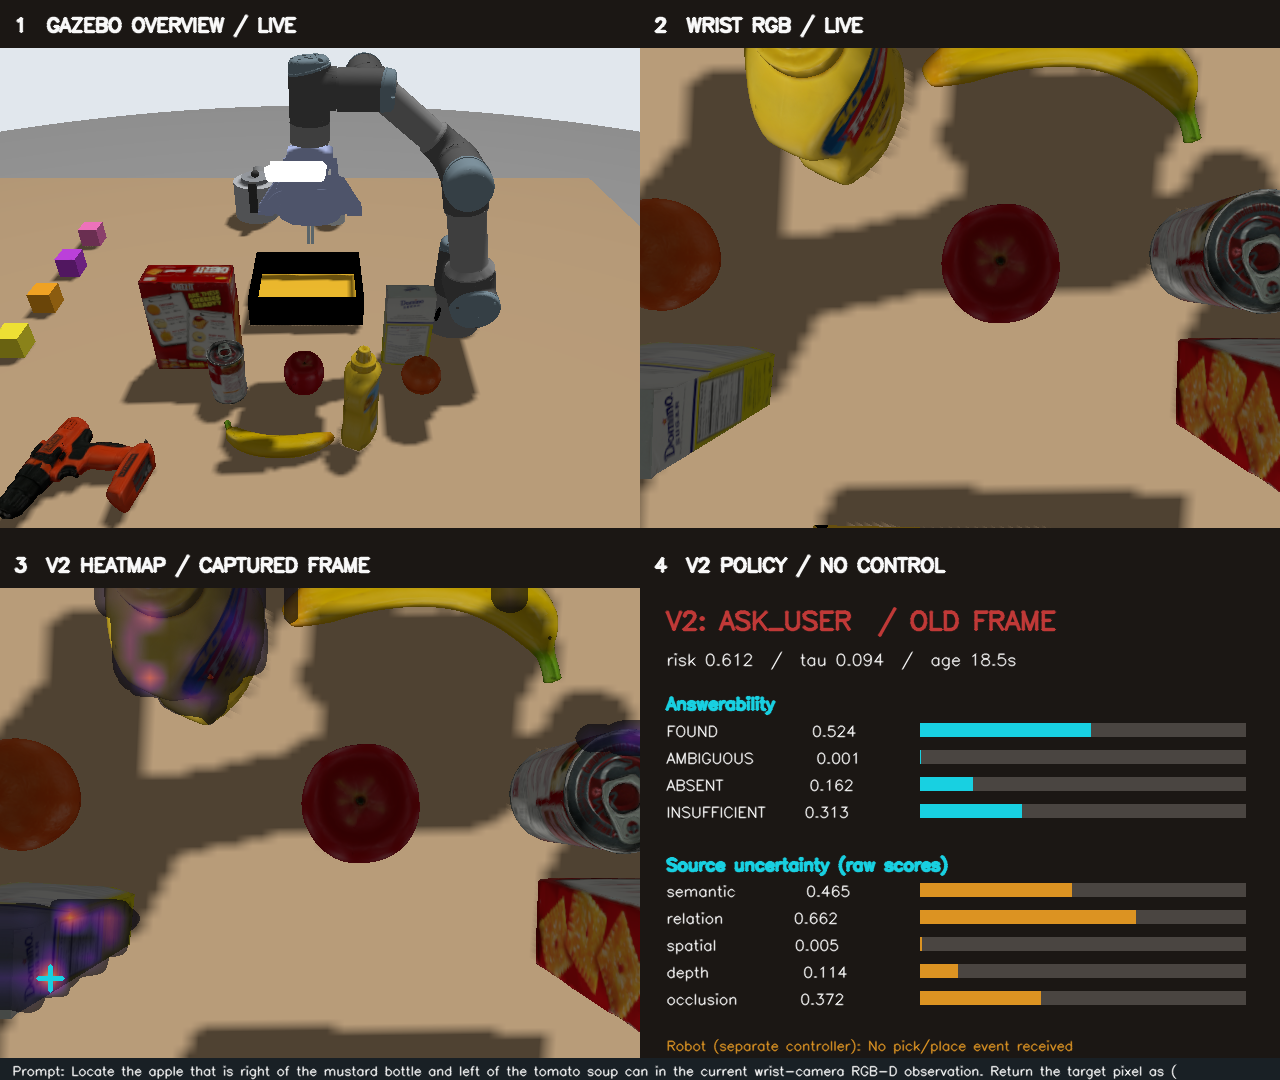
\includegraphics[width=\textwidth,height=0.70\textheight,keepaspectratio]{hinhanh/last_dashboard.png}
    \caption{Giao diện demo bốn ô: quan sát tổng thể, RGB camera cổ tay,
    heatmap trên khung suy luận và trạng thái policy.
    Ảnh minh họa có cảnh báo prediction cũ và không phát lệnh robot.}
    \label{fig:setup-live-dashboard}
    {\footnotesize Nguồn: ảnh dashboard đã lưu từ run Gazebo trong
    workspace. Đây là preview bố cục tùy chỉnh, không phải
    một sample Test-IID chính thức hay kết quả pick-and-place.\par}
\end{figure}

Overlay heatmap phải nằm trên \emph{ảnh đã dùng suy luận},
không đặt một điểm cũ lên ảnh live mới nếu camera hoặc
robot đã thay đổi. Panel hiển thị tuổi prediction để
người xem phân biệt cập nhật giao diện với cập nhật mô
hình. Dấu MAP ứng viên cũng phải khác điểm được cấp
cho hành động khi policy không chọn \texttt{EXECUTE}.

\subsection{Audit nhiều khung hình và kiểm tra vật đích độc lập}

Trước khi nối MoveIt, một run audit mới dùng pose camera
Test-IID và năm frame có timestamp riêng. Quy trình gồm
ba bước tách biệt: suy luận V2 rồi khóa prediction/
decision; kiểm tra vật đích bằng RGB-D không đọc nhãn;
cuối cùng evaluator mới mở semantic labels để chấm.

Checker RGB-D hiện có dành cho quả táo trong cảnh
cụ thể: kiểm tra một thành phần đỏ đủ lớn, tương
đối tròn, duy nhất theo điều kiện của checker và
depth phù hợp ở điểm ứng viên. Đây không phải bộ
nhận dạng độc lập đã được xác nhận cho mọi vật thể.
Nhãn Gazebo chỉ kiểm tra sau prediction, không
được dùng để chọn mục tiêu trước khi mô hình chạy.

\begin{figure}[htbp]
    \centering
    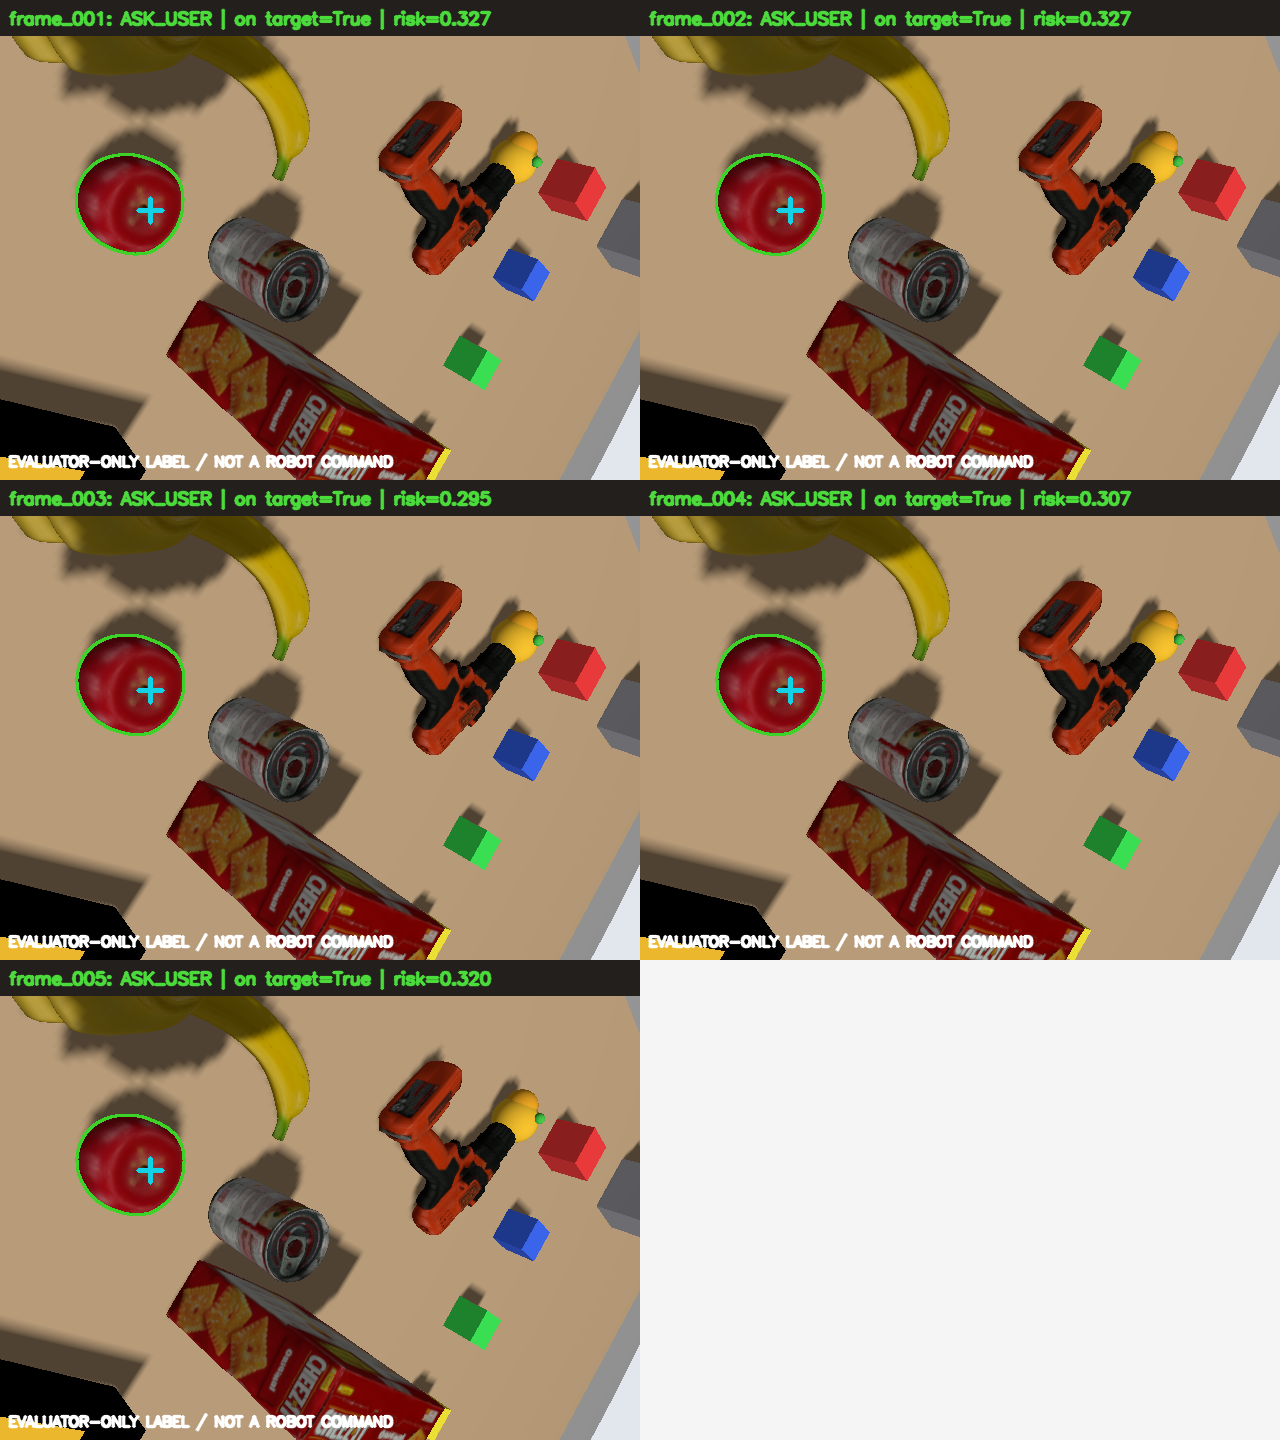
\includegraphics[width=\textwidth,height=0.74\textheight,keepaspectratio]{hinhanh/audit_montage.png}
    \caption{Audit năm khung hình ở pose camera Test-IID trên cảnh
    demo riêng. Các điểm ứng viên được đối chiếu với nhãn sau
    khi prediction đã khóa; policy vẫn trả về \texttt{ASK\_\allowbreak USER}.}
    \label{fig:setup-multiframe-audit}
    {\footnotesize Nguồn: capture, prediction lock và montage
    evaluator của run \texttt{iid\_\allowbreak pose\_\allowbreak audit} trong workspace.
    Không có chuyển động robot được phát từ run này.\par}
\end{figure}

Audit lưu riêng MAP, biến thiên điểm, kết quả checker RGB-D,
nhãn hậu kiểm, decision và trạng thái pre-handoff. Kết quả định lượng
được phân tích ở Chương~5. Khi diễn giải độ ổn định cần xét lượng tử hóa
ô $20\times20$ pixel; khi diễn giải risk cần xét khác biệt bố cục dù
pose camera giống Test-IID. Các kiểm tra này không thay thế đánh giá
sai số 3D hoặc xác nhận calibration trên miền demo mới.

\subsection{Ranh giới giữa demo nhận thức và thao tác}

Demo hiện không phát target hay trajectory từ V2
sang controller. MoveIt chưa nối vào run audit,
và không có robot motion được yêu cầu.
Log sự kiện của một controller lịch sử, nếu được
hiển thị trong dashboard, không tự trở thành bằng
chứng V2 điều khiển pick-and-place.

Để đánh giá thao tác cần thêm chuyển điểm sang
3D đúng TF, kiểm tra reachability/va chạm, chọn
tư thế gắp, điều khiển gripper và xác minh trạng
thái vật sau hành động. Khi đó mới định nghĩa
task success và số trial độc lập.
Chương này chỉ ghi nhận phần tích hợp đã có,
không dùng point-in-target thay cho task success.

\section{Khả năng tái lập và quy ước trình bày kết quả}
\label{sec:setup-reproducibility}

\subsection{Thứ tự tái lập từ artifact}

Để tái lập thí nghiệm từ đầu cần giữ thứ tự:
kiểm tra manifest/cache; huấn luyện trên train/dev;
khóa best; fit calibration riêng; khóa artifact;
capture/QC Test-IID; materialize; suy luận hai
hệ thống; join evaluator; tổng hợp metric và CI.
Thay đổi thứ tự có thể làm test ảnh hưởng ngược
đến chọn mô hình hoặc threshold.

Nếu chỉ tái lập hình/bảng từ kết quả hiện có,
không cần huấn luyện hoặc chạy lại suy luận.
Prediction, decision và evaluator manifest là
nguồn để tính thống kê. Bảng cấu hình lấy từ
config snapshot của run, không lấy một config
V3 đang mở trong IDE thay cho V2 đã báo cáo.

\subsection{Artifact cần giữ cùng mỗi kết quả}

{\setlength{\emergencystretch}{3em}
Mỗi run cần có config, seed/runtime, checkpoint
metadata và hash, history cùng prediction/evaluation
có sample ID. Bộ Test-IID giữ capture metadata,
QC report, dataset index, input/eval manifest
riêng, feature index và freeze lock.\par}


Ảnh minh họa phải gắn với sample hoặc run thực.
Mask ground-truth cần ghi là evaluator-only;
heatmap nội suy cần ghi độ phân giải dự đoán gốc;
ảnh RGB Gazebo không được ghi là ảnh chụp vật lý.
Các figure trong chương lấy từ file hiện có,
không dựng cảnh giả bằng ảnh sinh AI.

\subsection{Quy ước bảng theo phong cách bài báo}

Bảng dùng đường ngang phân cấp, không kẻ dọc,
caption trên bảng và nguồn/ghi chú phía dưới.
Số đếm được căn phải; đơn vị đặt trong heading;
tỉ lệ thống nhất thang $[0,1]$ hoặc phần trăm
và ghi rõ thang đang dùng. Metric tăng tốt hoặc
giảm tốt chỉ dùng mũi tên khi có bảng so sánh
định lượng thực sự.

Không in đậm một kết quả như “tốt nhất” nếu chưa
có cùng protocol và đủ đối chứng. Ô chưa có
artifact được ghi rõ chưa đánh giá, không dùng
0 để thay dữ liệu thiếu. Các CI phải đi kèm
đơn vị bootstrap là family và số lượt resampling.

\subsection{Tóm tắt thiết lập thực nghiệm}

Các tập vẫn có 320 family train, 80 dev, 200 calibration và 200 Test-IID, với năm variant mỗi family. Best V2 và Adapter đều được chọn trên dev; calibrator được fit sau freeze. RoboRefer, V2 và Adapter được đối chiếu trên cùng ảnh/câu lệnh. Grounding Adapter giữ nguyên V2; answerability và policy được đánh giá lại trên IID cũ, với CI cluster theo 200 family cho các thống kê đã bootstrap.

Các đối chứng ablation đầy đủ và thao tác robot
khép kín chưa có bằng chứng tương ứng trong
báo cáo chính; chúng được nêu như giới hạn.
Chương~5 sẽ trình bày số liệu hiệu quả, mức
khác biệt so baseline, calibration/selective
prediction, phân tầng và failure case theo
đúng thiết lập đã xác định ở chương này.
